\ifx\WithAttachments\undefined
  \def\WithAttachments{0}
\fi

\documentclass[10pt,letterpaper]{article}

\usepackage[utf8]{inputenc}
\usepackage[margin=0.6in]{geometry}
\usepackage{titlesec}
\usepackage{enumitem}
\usepackage{hyperref}
\usepackage{xcolor}
\usepackage{fontawesome5}
\usepackage{pdfpages}
\usepackage{pdflscape}
\usepackage{xstring}

% ==================== COLOR CONFIGURATION ====================

\definecolor{primary}{RGB}{30, 41, 59}
\definecolor{secondary}{RGB}{71, 85, 105}
\definecolor{accent}{RGB}{2, 132, 199}

\hypersetup{
    colorlinks=true,
    linkcolor=accent,
    urlcolor=accent
}

% ==================== TYPOGRAPHY ====================

\urlstyle{same}
\pagestyle{empty}

\titleformat{\section}
  {\large\bfseries\color{primary}}
  {}{0em}
  {}[\color{secondary}\titlerule\vspace{0.4em}]

\titlespacing*{\section}{0pt}{1.2em}{0.4em}

\setlist[itemize]{
    leftmargin=1.5em,
    noitemsep,
    topsep=0.2em,
    parsep=0.1em
}

% ==================== ATTACHMENT TOGGLE ====================

\newif\ifincludeattachments

\if\WithAttachments1
  \includeattachmentstrue
\else
  \includeattachmentsfalse
\fi

\begin{document}

% ============================================================
% HEADER
% ============================================================

\begin{center}

    {\LARGE\bfseries\color{primary} Satyam Awasthi} \\ \vspace{0.3em}
    {\color{secondary} Researcher \& Software Engineer} \\ \vspace{0.4em}
    \small 
    \faEnvelope~\href{mailto:satyam.aw@yahoo.com}{satyam.aw@yahoo.com} \ | \ 
    \faGlobe~\href{https://satyam-aw.github.io}{satyam-aw.github.io} \ | \ 
    \faGithub~\href{https://github.com/satyam-aw}{satyam-aw} \ | \ 
    \faOrcid~\href{https://orcid.org/0000-0002-6095-4303}{0000-0002-6095-4303} \ | \ 
    \faLinkedin~\href{https://linkedin.com/in/satyam-awasthi}{LinkedIn}  
    % Kanpur, IN \,$\cdot$\,
\end{center}

\vspace{0.35em}

% ============================================================
% RESEARCH SUMMARY
% ============================================================

\section*{Research Summary}

Computer Science researcher working on \textbf{neural interfaces}, \textbf{physiological sensing}, and \textbf{uncertainty-aware control}. Current work spans \textbf{EEG-based brain--computer interfaces} and \textbf{robust output-feedback model predictive control}.

% ============================================================
% RESEARCH INTERESTS
% ============================================================

\section*{Research Interests}

Neural Interfaces,
Brain--Computer Interfaces,
Physiological \& Wearable Sensing,
Human--Machine Interaction,
Machine Learning for Biosignals,
Robust State Estimation,
and Model Predictive Control.

% ============================================================
% RESEARCH EXPERIENCE
% ============================================================

\section*{Research Experience}

% ------------------------------------------------------------
% KOEHLER
% ------------------------------------------------------------

\noindent
\textbf{\href{https://www.imperial.ac.uk/autonomous-systems/}{Autonomous Systems Group}, Imperial College London}
\hfill Jul 2026 -- Present
\\
\textit{Research Collaboration}
\hfill
Advisor: \href{https://profiles.imperial.ac.uk/j.kohler}{Dr. Johannes K\"ohler}

\begin{itemize}

    \item Investigating \textbf{state-dependent estimation and tracking-error bounds}
    for nonlinear robust output-feedback MPC with state-dependent process and measurement uncertainty.

    \item Developing coupled observer and tracking-error tube propagation using
    \textbf{contraction-based certificates} for robust constraint tightening and
    uncertainty-aware trajectory planning.

\end{itemize}

\medskip

% ------------------------------------------------------------
% UCSB FOUR EYES
% ------------------------------------------------------------

\noindent
\textbf{\href{https://four-eyes.github.io/}
{Four Eyes Laboratory}, University of California, Santa Barbara}
\hfill Sep 2021 -- Jun 2023
\\
\textit{Graduate Researcher}
\hfill
Advisor:
\href{https://www.cs.ucsb.edu/~holl/}
{Prof. Tobias H\"ollerer};
Co-Advisor:
\href{https://beyelerlab.ucsb.edu/}
{Prof. Michael Beyeler}

\begin{itemize}

    \item Developed \textbf{EyeTTS}, an open-source framework for evaluating and
    calibrating eye tracking during mixed-reality locomotion, resulting in
    first-author publications at IEEE ISMAR Adjunct and IEEE VR Workshops.

    \item Designed human-subject experiments and analyzed
    \textbf{gaze-tracking accuracy, calibration drift, and motion-dependent sensing error}
    across multiple mixed-reality devices.

    \item Released a reproducible
    \href{https://github.com/satyam-aw/EyeTTS_Calibration-Framework}
    {\textbf{calibration framework}}
    and
    \href{https://github.com/satyam-aw/EyeTTS_Calibration-Framework/tree/main/participant-data}
    {\textbf{multi-device eye-tracking dataset}}
    containing gaze trajectories, calibration measurements, and locomotion data.

\end{itemize}

\medskip

% ------------------------------------------------------------
% IIT KGP ROBOTICS
% ------------------------------------------------------------

\noindent
\textbf{Autonomous Ground Vehicle \& Swarm Robotics Group,
IIT Kharagpur}
\hfill Jan 2016 -- Dec 2018
\\
\textit{Undergraduate Researcher}

\begin{itemize}

    \item Contributed to \textbf{Eklavya 6.0},
    IIT Kharagpur's autonomous ground vehicle that finished
    \textbf{Runner-Up} at the
    \textbf{Intelligent Ground Vehicle Competition (IGVC) 2018}.

    \item Developed perception and navigation components integrating
    LiDAR, IMU, GPS, vision-based perception, state estimation,
    and motion planning.

    \item Worked on decentralized multi-agent coordination using
    relative-pose estimation and communication over an ad-hoc mesh network.

\end{itemize}

% ============================================================
% PUBLICATIONS
% ============================================================

\section*{Publications}

\subsection*{Peer-Reviewed Conference Papers}

\noindent
\textbf{SmartWatch for Wall Writing:
Real-time Transcription of Wall Writing from Inertial Sensing}
\\
Snigdha Das,
\textbf{Satyam Awasthi},
Abdul Shamnar P,
Pradipta De,
Sandip Chakraborty,
and Bivas Mitra.
\\
\textit{COMSNETS}, 2022.
\\
\href{https://doi.org/10.1109/COMSNETS53615.2022.9668531}
{\color{accent}\footnotesize
DOI: 10.1109/COMSNETS53615.2022.9668531}

\vspace{-0.5em}

\subsection*{Workshop \& Poster Publications}

\noindent
\textbf{Eye Tracking Performance in Mobile Mixed Reality}
\\
\textbf{Satyam Awasthi},
Vivian Ross,
Sydney Lim,
Michael Beyeler,
and Tobias H\"ollerer.
\\
\textit{IEEE VR Workshops (VRW)}, 2024.
\\
\href{https://doi.org/10.1109/VRW62533.2024.00321}
{\color{accent}\footnotesize
DOI: 10.1109/VRW62533.2024.00321}

\medskip

\noindent
\textbf{EyeTTS:
Evaluating and Calibrating Eye Tracking for Mixed-Reality Locomotion}
\\
\textbf{Satyam Awasthi},
Vivian Ross,
Michael Beyeler,
and Tobias H\"ollerer.
\\
\textit{IEEE ISMAR Adjunct}, 2023.
\\
\href{https://doi.org/10.1109/ISMAR-Adjunct60411.2023.00104}
{\color{accent}\footnotesize
DOI: 10.1109/ISMAR-Adjunct60411.2023.00104}

% ============================================================
% SELECTED RESEARCH PROJECTS
% ============================================================

\section*{Selected Research Projects}

% ------------------------------------------------------------
% EEG BCI
% ------------------------------------------------------------

\noindent
\textbf{
\href{https://satyam-aw.github.io/projects/bci_maze/}
{EEG-Based BCI for 3D Navigation}}
\hfill 2026 -- Present
\\
\textit{Independent Neural Interface Project}

\begin{itemize}

    \item Developing a
    \textbf{4-channel EEG acquisition and decoding pipeline}
    for real-time control of an interactive 3D navigation environment.

    \item Building an initial
    \textbf{SSVEP-based intent-decoding system}
    using neural-signal preprocessing and
    spectral / correlation-based features
    for discrete movement commands.

    \item Investigating confidence thresholds and temporal evidence
    accumulation to characterize the trade-off between
    \textbf{decoding reliability and command latency}.

\end{itemize}

% ------------------------------------------------------------
% SMARTWATCH
% ------------------------------------------------------------

\noindent
\textbf{
\href{https://doi.org/10.1109/COMSNETS53615.2022.9668531}
{SmartWatch for Wall Writing}}
\hfill 2019 -- 2022
\\
\textit{Wearable Inertial Sensing for Human--Computer Interaction}

\begin{itemize}

    \item Contributed to a wearable sensing system for
    \textbf{real-time transcription of free-form wall writing}
    from smartwatch inertial measurements.

    \item Explored the use of human wrist-motion signals as an
    unobtrusive input modality for recognizing physical writing gestures.

\end{itemize}

% ------------------------------------------------------------
% JITTERNOT
% ------------------------------------------------------------

\noindent
\textbf{
\href{https://satyam-aw.github.io/projects/jitternot/}
{JitterNot}}
\hfill Jan 2022 -- Mar 2022
\\
\textit{Learning-Based Model Predictive Control for Adaptive Video Streaming
(UCSB)}

\begin{itemize}

    \item Developed an LSTM-based predictor for network throughput
    to support closed-loop decisions under non-stationary network dynamics.

    \item Designed a receding-horizon
    \textbf{model predictive control (MPC)}
    framework for adaptive bitrate selection under bandwidth constraints.

\end{itemize}

% ------------------------------------------------------------
% HAR
% ------------------------------------------------------------

\noindent
\textbf{
\href{https://satyam-aw.github.io/projects/in_motion_har_deepconvlstm/}
{In Motion --- Wearable Human Activity Recognition}}
\hfill Nov 2019
\\
\textit{DeepConvLSTM Modeling of Inertial Sensor Signals (IIT Kharagpur)}

\begin{itemize}

    \item Designed a streaming inference pipeline for
    \textbf{high-frequency IMU signals}
    enabling temporal human-activity classification.

    \item Implemented a DeepConvLSTM architecture combining
    convolutional feature extraction with recurrent temporal modeling
    of wearable sensor sequences.

\end{itemize}

% ============================================================
% EDUCATION
% ============================================================

\section*{Education}

\noindent
\textbf{University of California, Santa Barbara (UCSB)}
\hfill Santa Barbara, CA
\\
\textit{M.S. in Computer Science (GPA: 3.91/4.00)}
\hfill Sep 2021 -- Jun 2023

\medskip

\noindent
\textbf{Indian Institute of Technology, Kharagpur (IIT Kharagpur)}
\hfill Kharagpur, India
\\
\textit{B.Tech. in Electrical Engineering,
Minor in Computer Science (GPA: 8.98/10.0)}
\hfill Jul 2016 -- Jul 2020

% ============================================================
% INDUSTRY EXPERIENCE
% ============================================================

\section*{Industry Experience}

\noindent
\textbf{Intuit Inc}
\hfill Mountain View, CA
\,$\cdot$\,
Mar 2024 -- Jan 2026
\\
\textit{Software Engineer 2}

\begin{itemize}

    \item Built
    \href{https://satyam-aw.github.io/projects/intuit_generative_ui/}
    {dual-stage agent pipelines}
    for intent routing, structured tool execution,
    and generative user-interface composition.

    \item Developed production platform infrastructure supporting
    large-scale client applications and internal developer workflows.

\end{itemize}

\noindent
\textbf{Yahoo Inc}
\hfill Mountain View, CA
\,$\cdot$\,
Apr 2023 -- Nov 2023
\\
\textit{Software Dev Engineer II (IC3)}

\begin{itemize}

    \item Developed production Android systems for Yahoo Mail,
    including data-driven inbox commerce and expense-management features.

\end{itemize}

\noindent
\textbf{Coupang Global LLC}
\hfill Mountain View, CA
\,$\cdot$\,
Jun 2022 -- Sep 2022
\\
\textit{Software Engineering Intern}

\begin{itemize}

    \item Developed user-facing search and product-discovery features
    for Coupang's Android commerce platform.

\end{itemize}

\noindent
\textbf{Samsung Research Institute}
\hfill Noida, India
\,$\cdot$\,
Sep 2020 -- Sep 2021
\\
\textit{Software Engineer (CL 2)}

\begin{itemize}

    \item Developed Android platform and device applications involving
    media processing, privacy, and isolated user-storage architectures.

\end{itemize}

% ============================================================
% TEACHING
% ============================================================

\section*{Teaching}

\noindent
\textbf{University of California, Santa Barbara}
\hfill Santa Barbara, CA
\\
\textit{
\href{https://satyam-aw.github.io/teaching/}
{Graduate Teaching Assistant}}
\hfill Sep 2021 -- Jun 2023

\begin{itemize}

    \item Led instructional labs, developed programming assignments,
    and supported senior capstone teams across
    CS189 (Capstone),
    CS184 (Android),
    CS24 (C++ Data Structures),
    and CS16 (Problem Solving).

\end{itemize}

% ============================================================
% TECHNICAL SKILLS
% ============================================================

\section*{Technical Skills}

\noindent
\textbf{Programming:}
Python, C++, MATLAB, Java, Kotlin

\medskip

\noindent
\textbf{Machine Learning \& Signal Processing:}
PyTorch, NumPy/SciPy, OpenCV,
Time-Series Modeling, Wearable/Inertial Signal Processing

\medskip

\noindent
\textbf{Control \& Estimation:}
Model Predictive Control (MPC), Robust MPC,
Contraction-Based Methods, State Estimation (EKF),
Sensor Fusion, Motion Planning

\medskip

\noindent
\textbf{Robotics \& Interactive Systems:}
ROS/ROS2, Gazebo, RViz, Unity, OpenGL

\medskip

\noindent
\textbf{Developer Tools:}
Git

% ============================================================
% ACADEMIC SERVICE
% ============================================================

\section*{Academic Service \& Peer Review}

\noindent
\textbf{Peer Reviewer, UIST 2024}
\\
\textit{ACM Symposium on User Interface Software and Technology}

\begin{itemize}

    \item Reviewed submissions on interactive systems,
    spatial tracking, and interface hardware.

\end{itemize}

% ============================================================
% OPTIONAL TRANSCRIPT ATTACHMENTS
% ============================================================

\clearpage

\ifincludeattachments

    \newgeometry{margin=0pt}

    \begin{landscape}
        \thispagestyle{empty}
        \noindent
        \centering
        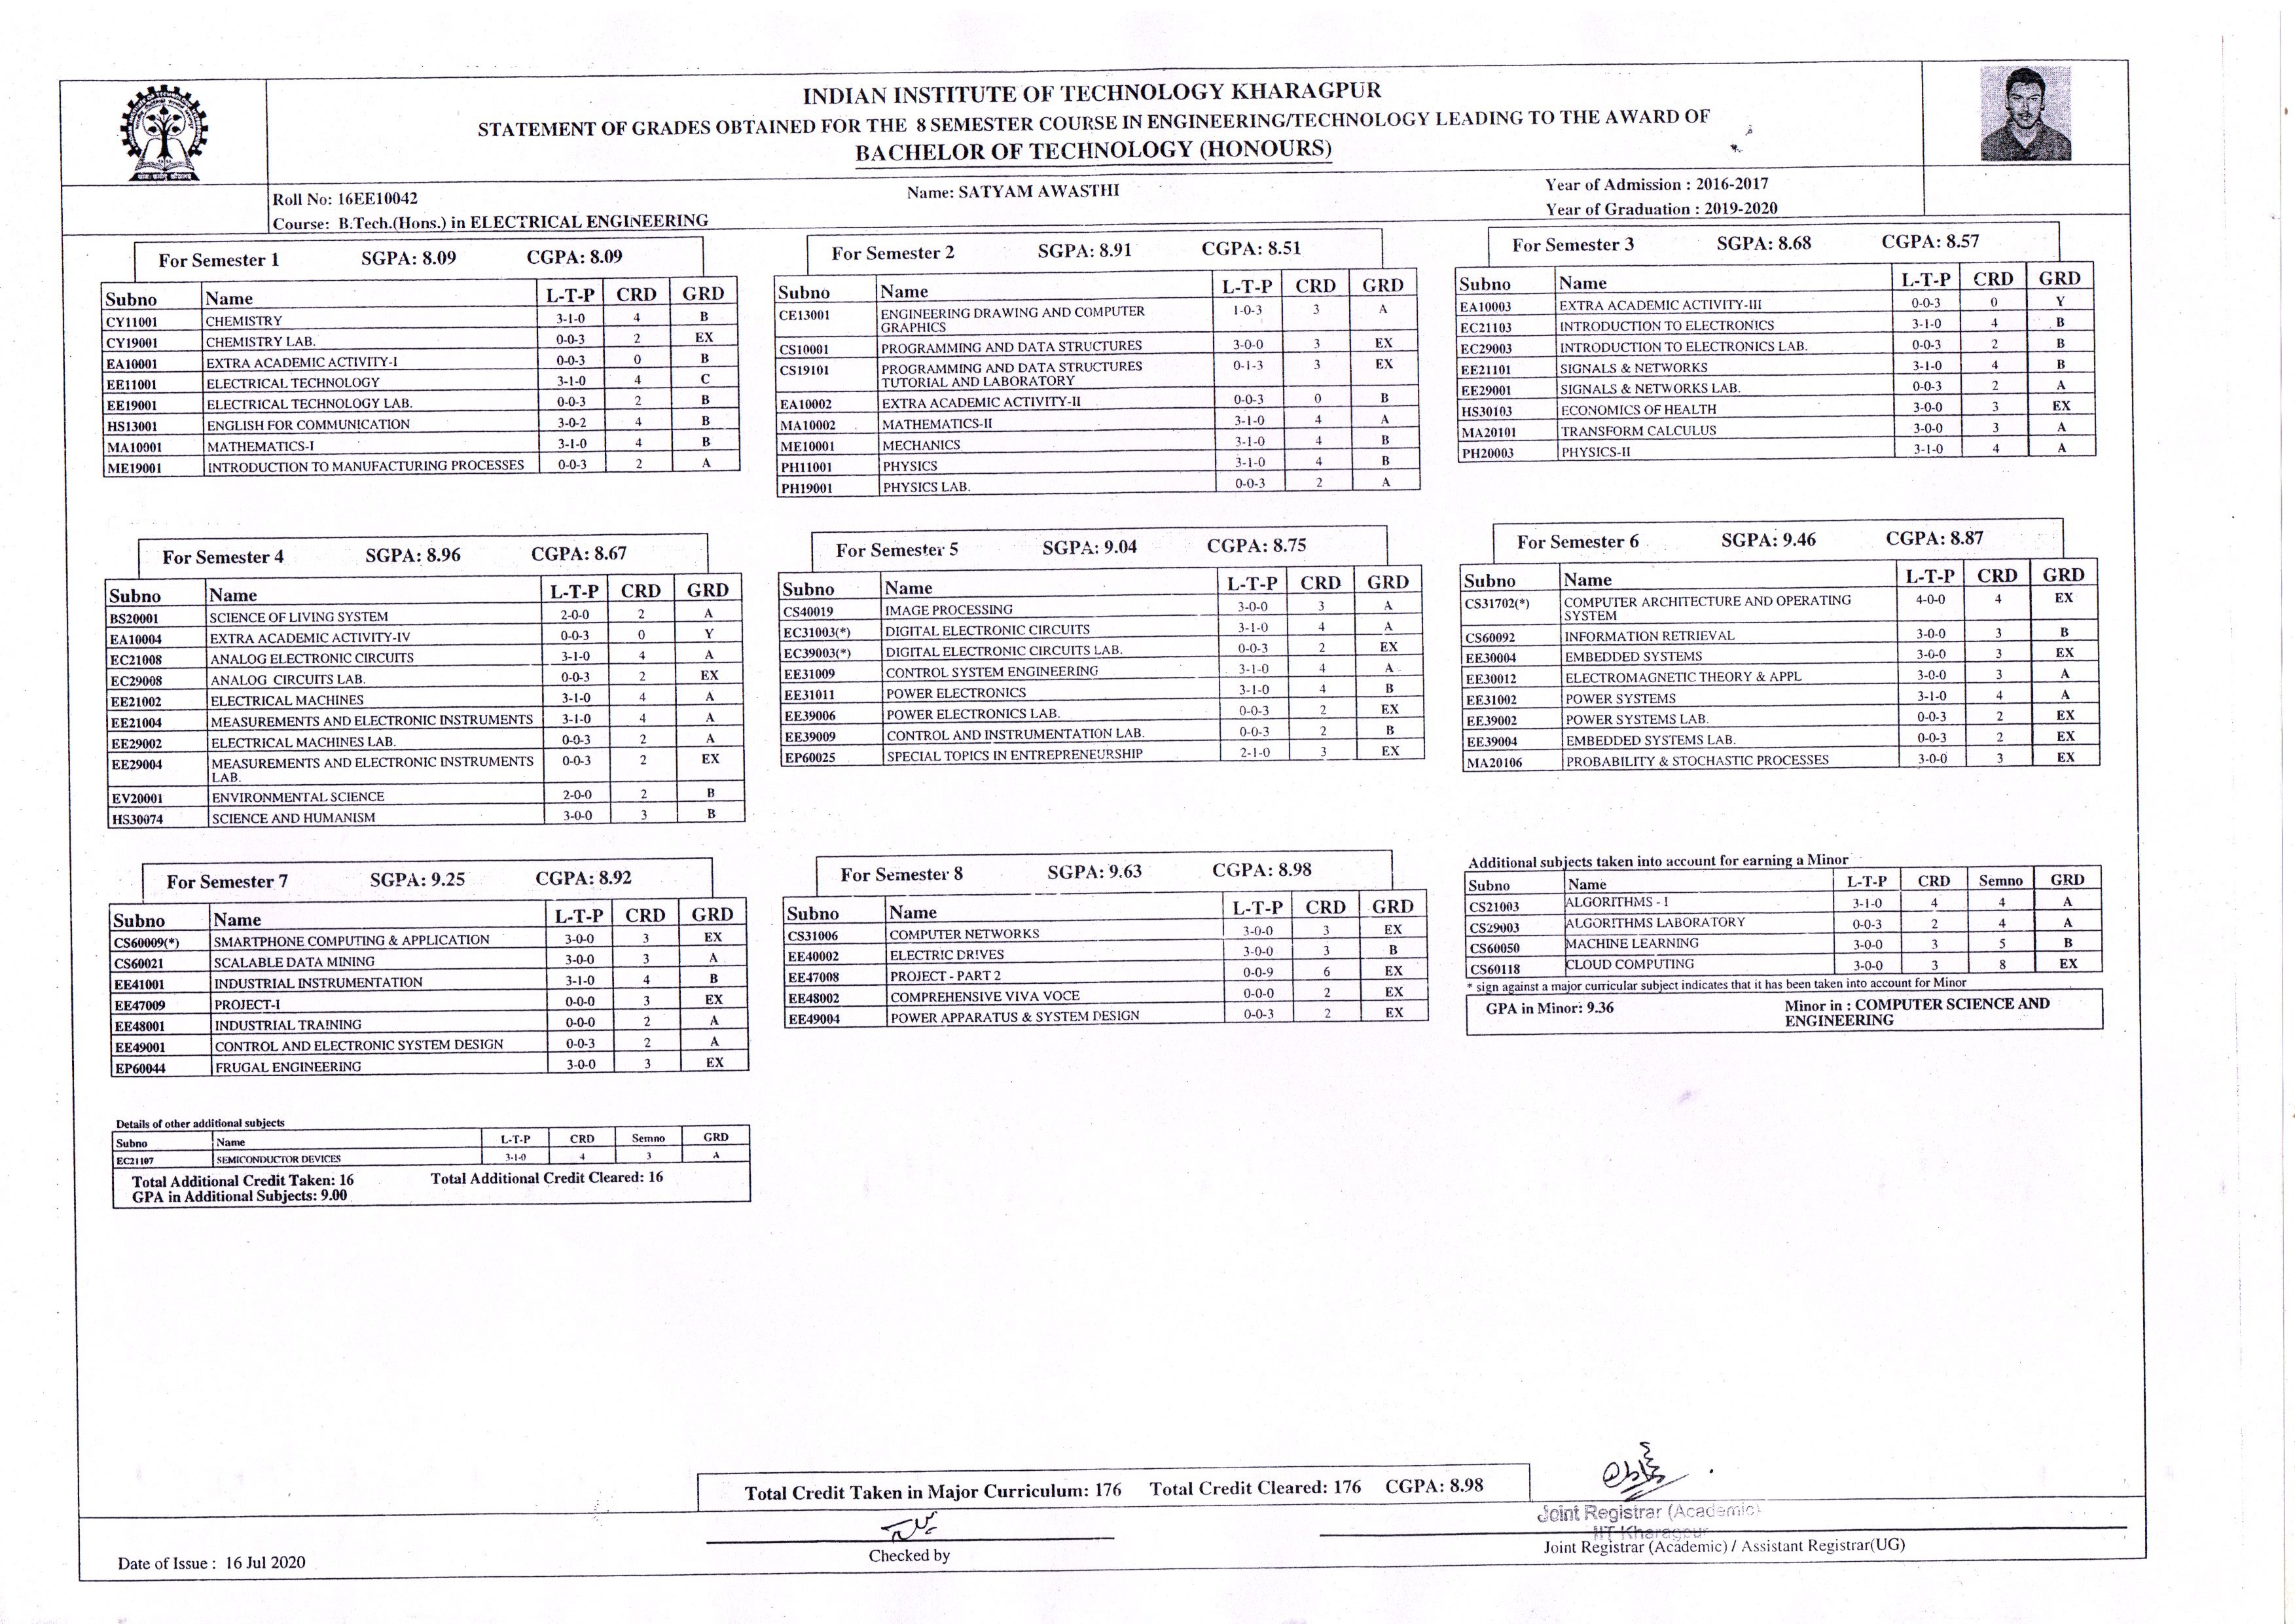
\includegraphics[
            width=\linewidth,
            height=\textheight,
            keepaspectratio
        ]{transcripts/kgp_transcript_full_TWCTPV1N.jpg}
    \end{landscape}

    \clearpage
    \restoregeometry

    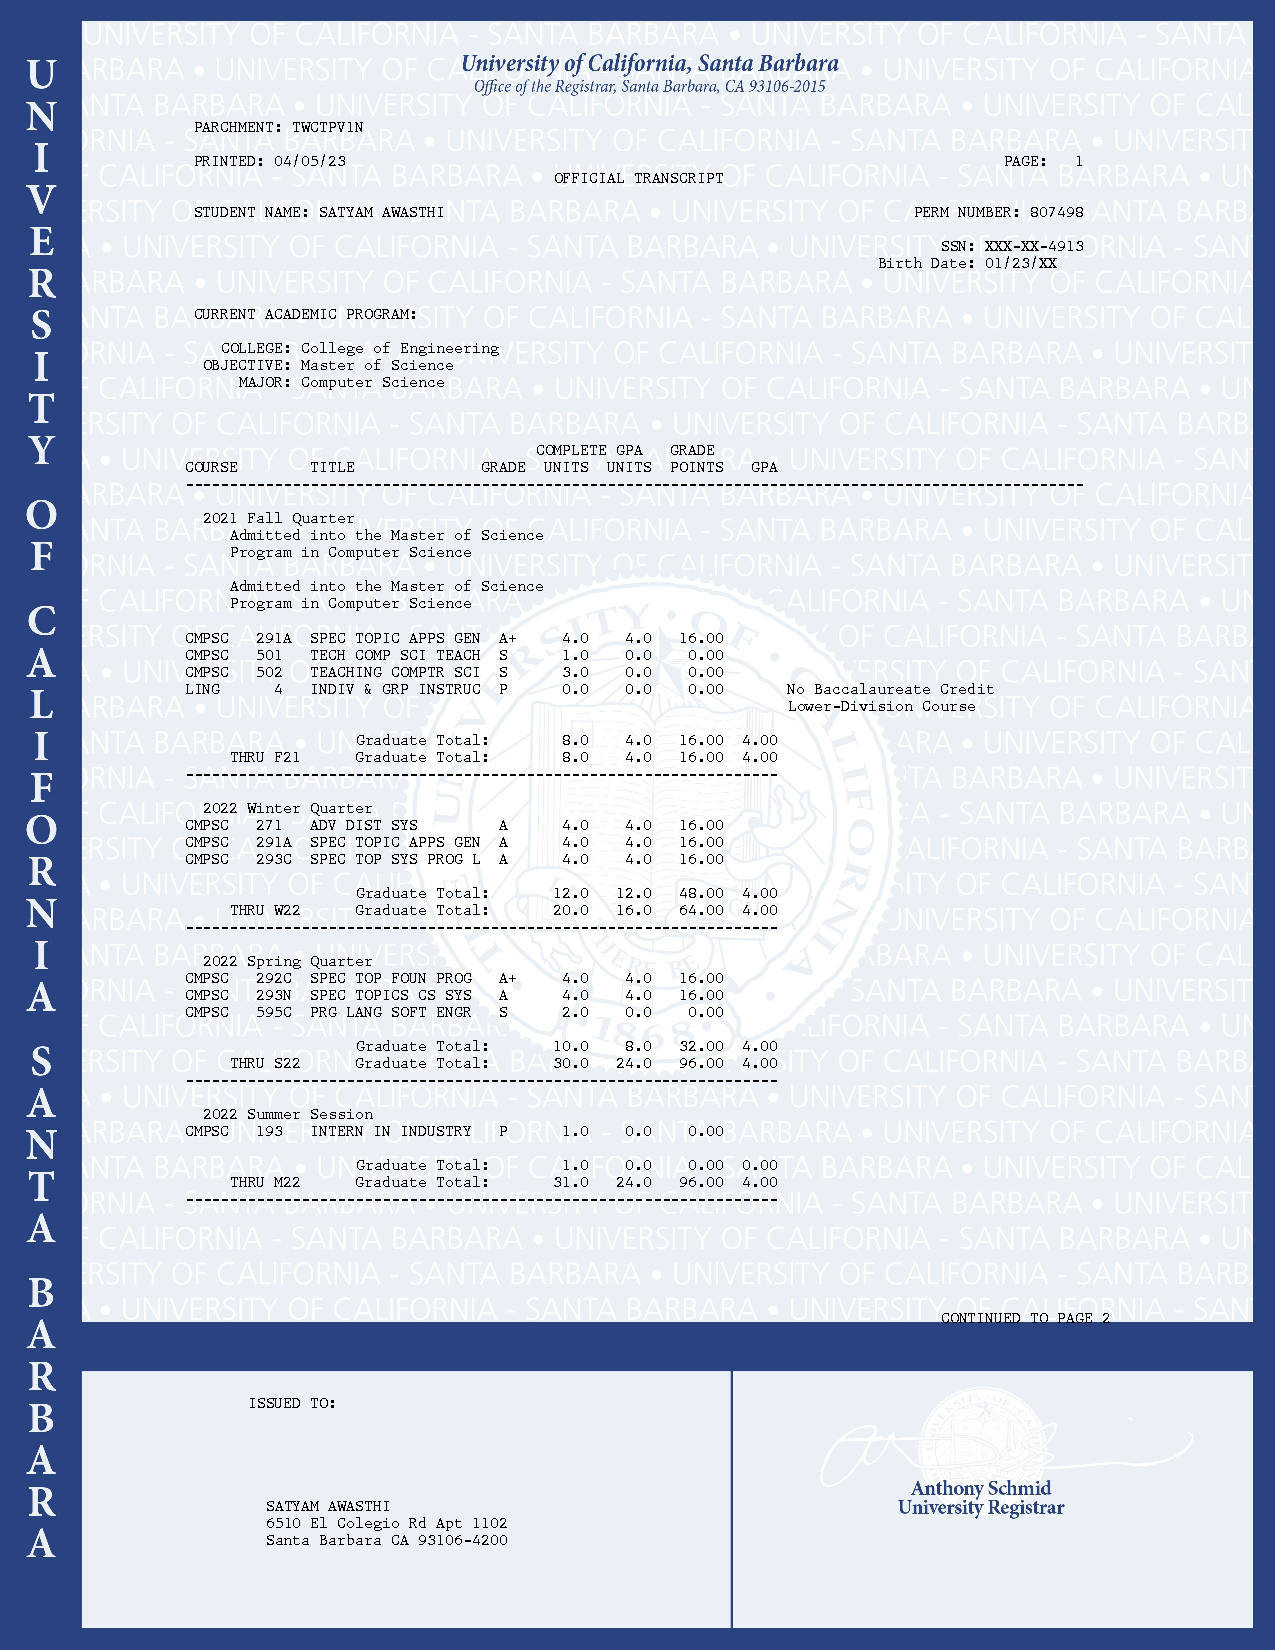
\includepdf[
        pages=-
    ]{transcripts/official_transcript_ucsb_TWCTPV1N.pdf}

\fi

\end{document}